\documentclass{article}
\setlength{\textheight}{9.3in}
\setlength{\textwidth}{6.68in}
\setlength{\oddsidemargin}{-.20in}
\setlength{\topmargin}{-.25in}
\setlength{\headsep}{10mm}
\pagestyle{myheadings}
\usepackage{graphics}
\usepackage{epsfig}
\usepackage{multicol}
\title{\hrule \vspace{0.3cm}MLE from a Competing Risks Model of an Exponential Failure and a Lognormal Survival}
\date{10 November 2010}
\author{Nikola Chochkov, MSc Statistics, Humboldt University Berlin}
\begin{document}
\maketitle
\hrule
\section{Introduction.}
\subsection{Assumptions.}
\indent \indent Two usage-measured lifetime random variables are discussed in a fixed-time life test. The items under study are considered to accumulate usage independently and with a different rate. The survival population is considered \textit{Lognormally distributed} (with parameters $\mu$ and $\sigma$), while the failure popoulation - \textit{Exponential} (with parameter $\lambda$). 
\\ 
\\ \indent An estimation of the parameter vector ($\lambda$, $\mu$, $\sigma$)$'$ is sought using all usage data collected (from both survival and failure cases) 
\begin{itemize}
\item $\eta \sim Lognormal$ 
\item $\psi \sim Exponential$
\item $f_\eta(x) = \frac{1}{x \sigma \sqrt{2 \pi}} e^{-\frac{\left( \ln x - \mu \right)^2}{2\sigma^2}} = \frac{1}{x \sigma} \phi \left( \frac{\ln x - \mu}{\sigma} \right) $ is the \textit{probability densitiy function} of the Lognormal distribution, with $\phi$ being the density function of the Standard Normal Distribution
\item $\overline F_\eta(x) = 1 - \frac{1}{\sqrt{2 \pi}} e^{-\frac{\left( \ln x - \mu \right)^2}{2\sigma^2}} = \overline \Phi \left(\frac{\ln x - \mu}{\sigma}\right)$ is its \textit{survival function}, with $\overline\Phi$ being the survival function of the Standard Normal Distribution
\item $f_\psi(x) = \lambda e^{- \lambda x}$ is the \textit{pdf} of the Exponential distribution 
\item $\overline F_\psi(x) = e^{- \lambda x}$ is its \textit{survival function}
\item $N_f = \{i : x_i\ is\ failed \}$ and $n_f  = \# N_f$ (i.e. number of failures) 
\item $N_s = \{i : x_i\ is\ survived \}$ and $n_f  = \# N_s$ (i.e. number of survivals)
\item $n$ is the total number of units under test ($n = n_f + n_s$)
\item $\textbf{x}$ is the data vector and $\textbf{x} = \left[ \textbf{x}^f, \textbf{x}^s \right] = \left[ x_1^f, ... , x_{n_f}^f, x_1^s, ... , x_{n_s}^s \right] $, where:
\item $\textbf{x}^f$ is the data for failed items, $\textbf{x}^f = \left[ x_1^f, ... , x_{n_f}^f \right] $
\item $\textbf{x}^s$ is the data for survived items, $\textbf{x}^s = \left[ x_1^s, ... , x_{n_s}^s \right] $
\item $\lambda, \mu, \sigma, x > 0$
\end{itemize}
\subsection{Maximum Likelihood Method.}
\indent \indent The Likelihood function is given by (since $\eta$ and $\psi$ are independent):
\begin{eqnarray}
\delta (\lambda, \mu, \sigma) \sim P[\psi < \eta | Fail] * P[\eta < \psi | Surv] = f_\psi(x | F)\overline F_\eta(x | F) * f_\eta(x | S) \overline F_\psi(x | S) 
\end{eqnarray}
\begin{eqnarray}
L(\lambda, \mu, \sigma | \textbf{x}) &=& \prod_{i \in N_f} \left[ f_\psi \left( x_i^f \right) \overline F_\eta \left( x_i^f \right) \right]\prod_{i \in N_s} \left[ f_\eta \left( x_i^s \right) \overline F_\psi \left( x_i^s \right) \right]
\end{eqnarray}
\indent Now from the above we can derive the Log Likelihood:
\begin{eqnarray}
LogL = L^*(\lambda, \mu, \sigma | \textbf{x}) &=& \sum_{i \in N_f} \ln \left[ f_\psi(x_i^f) \right] + \sum_{i \in N_f} \ln \left[ \overline F_\eta(x_i^f) \right] + \sum_{i \in N_s} \ln \left[ f_\eta (x_i^s) \right] + \sum_{i \in N_s} \ln \left[ \overline F_\psi(x_i^s) \right]
\end{eqnarray}
\indent And if we apply the above notation and rework:
\begin{eqnarray}
L^*(\lambda, \mu, \sigma | \textbf{x}) &=& N_f \ln \lambda - \lambda \sum_{i = 1}^n x_i + \sum_{i \in N_f} \ln \overline \Phi \left( \frac{\ln x_i^f - \mu}{\sigma} \right) - \sum_{i \in N_s} \ln \sigma x_i^s + \sum_{i \in N_s} \ln \phi \left( \frac{\ln x_i^s - \mu}{\sigma} \right)
\end{eqnarray}
\indent The MLE estimators $\left(\hat \lambda, \hat \mu, \hat \sigma \right)$ would be the ones that turn $L^*$ into a minimum, so now we need to compute the \textit{Gradient} vector and \textit{Hessian} matrix in order to find them. Furthermore we would like to show that the estimators have the \textit{consistency} property.\\ 
\subsection{First order derivatives of $L^*$ w.r.t $\left(\lambda, \mu, \sigma \right)$}
\indent Let's denote: $z_i^{f,s} = \frac{\left(\ln x_i^{f,s} - \mu \right)}{\sigma}$. Then we derive: 
\begin{eqnarray}
\frac{\partial z}{\partial \mu} = - \frac{1}{\sigma} , \frac{\partial z} {\partial \sigma} = - \frac{1}{\sigma}z , \frac{\partial \phi}{\partial \sigma} = \frac{1}{\sigma}\phi z^2 , \frac{\partial \phi}{\partial \mu} = \frac{1}{\sigma}\phi z 
\end{eqnarray} 
\begin{eqnarray}
\frac{\partial L^*(\lambda, \mu, \sigma | \textbf{x}) }{\partial \lambda} &=& \frac{n_f}{\lambda} - \sum_{i = 1}^n x_i 
\end{eqnarray} 
\begin{eqnarray}
\frac{\partial L^*(\lambda, \mu, \sigma | \textbf{x}) }{\partial \mu} &=& \frac{1}{\sigma}\sum_{i \in N_f} \frac{\phi \left( z_i^f \right)}{\overline \Phi \left( z_i^f \right)} + \frac{1}{\sigma}\sum_{i \in N_s}z_i^s 
\end{eqnarray} 
\begin{eqnarray}
\frac{\partial L^*(\lambda, \mu, \sigma | \textbf{x}) }{\partial \sigma} &=& \frac{1}{\sigma} \sum_{i \in N_f} \frac{\phi \left( z_i^f \right) z_i^f }{\overline \Phi \left( z_i^f \right)} + \frac{1}{\sigma}\sum_{i \in N_s} (z_i^s)^2 - \frac{n_s}{\sigma} 
\end{eqnarray} 
\subsection{Second order derivatives of $L^*$ w.r.t $\left(\lambda, \mu, \sigma \right)$}\
\indent Let's denote again: $z_i^{f,s} = \frac{\left(\ln x_i^{f,s} - \mu \right)}{\sigma}$. Then we derive: 
\begin{eqnarray}
\frac{\partial^2 L^*(\lambda, \mu, \sigma | \textbf{x}) }{\partial \lambda^2} &=& - \frac{n_f}{\lambda ^ 2} 
\end{eqnarray} 
\begin{eqnarray}
\frac{\partial^2 L^*(\lambda, \mu, \sigma | \textbf{x}) }{\partial \mu^2} &=& \frac{1}{\sigma^2}\sum_{i \in N_f} \left[ \frac{\phi \left( z_i^f \right)}{\overline \Phi \left( z_i^f \right)}\left( 1 + \frac{\phi \left( z_i^f \right)}{\overline \Phi \left( z_i^f \right)} \right) z_i^f \right] - \frac{1}{\sigma^2} 
\end{eqnarray} 
\begin{eqnarray}
\frac{\partial^2 L^*(\lambda, \mu, \sigma | \textbf{x}) }{\partial \mu \partial\sigma} &=& \frac{1}{\sigma^2} \sum_{i \in N_f} \frac{\phi \left( z_i^f \right)}{\overline \Phi \left( z_i^f \right)} + \frac{1}{\sigma^2}\sum_{i \in N_f} \left[ \frac{\phi \left( z_i^f \right)}{\overline \Phi \left( z_i^f \right)}\left( 1 + \frac{\phi \left( z_i^f \right)}{\overline \Phi \left( z_i^f \right)} \right) z_i^f \right] - \frac{2}{\sigma^2}\sum_{i \in N_s} z_i^s 
\end{eqnarray} 
\begin{eqnarray}
\frac{\partial^2 L^*(\lambda, \mu, \sigma | \textbf{x}) }{\partial \sigma^2} &=& \frac{1}{\sigma^2} \sum_{i \in N_f} \left[ \frac{\phi (z_i) z_i^3}{\overline \Phi} - 2\frac{\phi(z_i)z_i}{\overline \Phi} - \frac{\phi^2(z_i) z_i^2}{\overline\Phi ^2} \right] - \frac{3}{\sigma^2}\sum_{i \in N_s} z_i^2 + \frac{n_s}{\sigma^2}
\end{eqnarray} 
\section{Simulation Studies}
\subsection{4 different sets of true parameter used to generate test items data. Number of tested items $n$ = 1000}
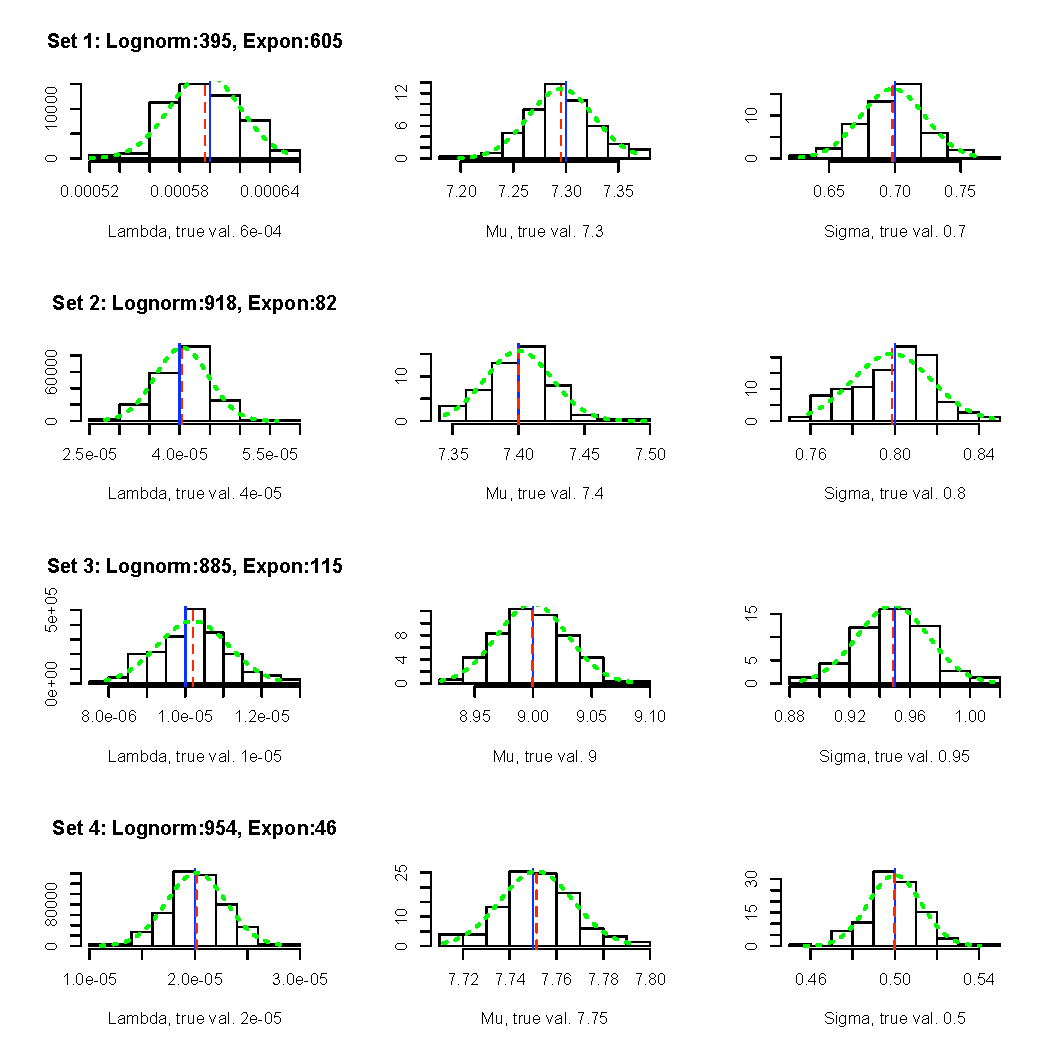
\includegraphics{Diagram1.pdf}
\subsection{The same true parameter sets, but increased $n$ = 2000}
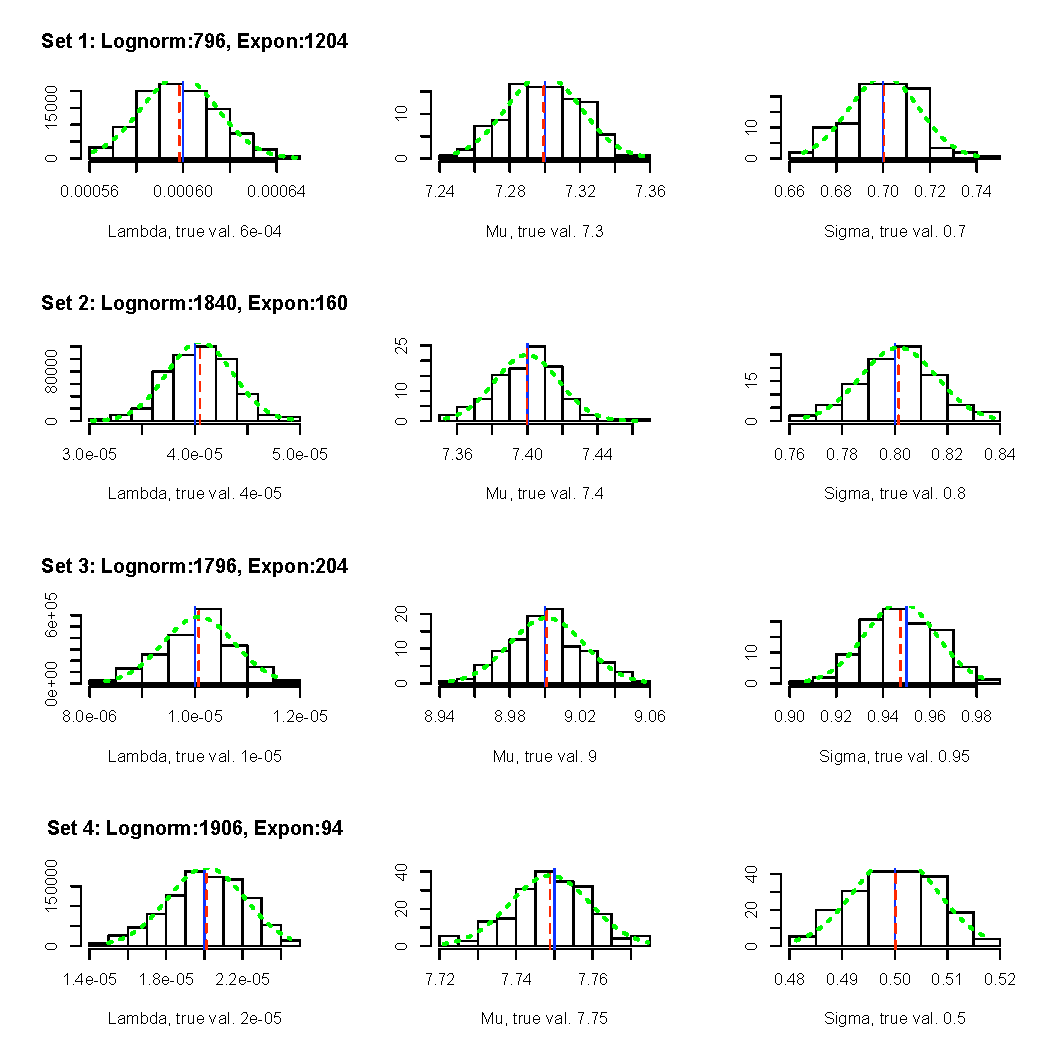
\includegraphics{Diagram2.pdf}
\section{Maximum Likelihood Estimators' properties.}
\subsection{Normality of the estimators.} This can be seen from the results from 4 simulation sets of true value parameters. 1000 items under study, 150 repetitions for each parameter set. Diagram 1.  \\
\subsection{Consistency of the estimators.} Simulations were done with the same parameter sets but with 2000 items under study, 150 simulation repetitions. Diagram 2.\\
\section{Next steps.}
Check the properties of the Variance Covariance matrix, Score, and perform more simulations on other true parameter sets and with more repetitions.
\end{document}

